% =============================================================================
%  The G-transform on the two-sphere  --  A0 landscape poster
%  Reading order is numbered 1-7 across the four columns.
% =============================================================================
\documentclass[landscape,a0paper,fontscale=0.34]{baposter}

\usepackage{graphicx}
\graphicspath{{figures/}{./}}
\usepackage{hyperref}
\hypersetup{colorlinks,citecolor=blue,filecolor=blue,linkcolor=blue,urlcolor=blue}
\usepackage{amsmath,amssymb,mathtools}
\usepackage{booktabs}
\usepackage{colortbl}
\usepackage{enumitem}
\usepackage{palatino}
\usepackage[font=small,labelfont=bf]{caption}
\usepackage{tikz}
\usepackage{tikz-3dplot}
\usepackage{tikz-cd}
\usetikzlibrary{arrows.meta,calc,positioning}

\newcommand{\Sph}{\mathbb S}
\newcommand{\cH}{\mathcal H}
% \newcommand{\cH}{\ensuremath{\mathcal{H}}}
\newcommand{\Cinf}{C^\infty}
\newcommand{\odd}{\mathrm{odd}}
\newcommand{\even}{\mathrm{even}}
\newcommand{\cG}{\mathcal G}
\newcommand{\cF}{\mathcal F}
\newcommand{\SO}{\mathrm{SO}}
\newcommand{\norm}[1]{\left\lVert #1\right\rVert}
\newcommand{\inner}[2]{\left\langle #1,#2\right\rangle}

% --- palette ----------------------------------------------------------------
\definecolor{blue}{rgb}{0.0,0.22,1}
\definecolor{softblue}{rgb}{0.95,0.97,1.0}
\definecolor{verysoftblue}{rgb}{0.985,0.99,1.0}
\definecolor{circ}{rgb}{0.05,0.24,0.55}      % great circles
\definecolor{accent}{rgb}{0.86,0.33,0.02}    % gradient vector
\definecolor{keep}{rgb}{0.90,0.96,0.90}      % "isomorphism" cells
\definecolor{drop}{rgb}{0.94,0.94,0.94}      % "kernel" cells

% caption style used under the two geometry figures
\newcommand{\figcap}[2]{\par\vspace{0.35em}%
  \begin{minipage}{0.94\linewidth}\small\textbf{#1}~#2\end{minipage}}

\begin{document}
\begin{poster}
{
headerborder=closed,
colspacing=1em,
bgColorOne=white,
bgColorTwo=white,
borderColor=blue,
headerColorOne=black,
headerColorTwo=blue,
headerFontColor=white,
boxColorOne=white,
textborder=roundedleft,
eyecatcher=true,
headerheight=0.105\textheight,
headershape=roundedright,
headerfont=\Large\bf\textsc,
linewidth=2pt
}
{\IfFileExists{UoM_logo.png}{
\includegraphics[height=6em]{UoM_logo.png}}{\rule{0pt}{6em}\hspace{7.5em}}}
{\bf\textsc{The Gunk $\cG$-Transform on the Sphere}\vspace{0.28em}\\[-0.15em]\large Geometry, spherical harmonics and inversion}
{\textsc{Rory Yarr \hspace{1.2cm} Supervisor: Volker Schlue \hspace{1.2cm} The University of Melbourne}}
{\IfFileExists{UoM_logo.png}{
\includegraphics[height=6em]{UoM_logo.png}}{\rule{0pt}{6em}\hspace{7.5em}}}

% =============================================================================
% 1. FUNK  (column 0, top)
% =============================================================================
% \subsection{1}
\headerbox{\textcolor{white}{1.} The Funk transform}{name=funk,column=0,row=0}{
In 1911 Paul Funk introduced the following transform over the sphere.
For $\omega\in\Sph^2$ and $f\in C^\infty(\Sph^2)$ let
\vspace{-0.9em}
\[\gamma_\omega = \{\sigma\in \Sph^2:\omega\cdot \sigma\}=0,\vspace{-0.8em} \]
be the great circle from $\omega$. Then the \emph{Funk transform} is 
\vspace{-1.1em}
\[ (\cF f)(\omega)=\int_{\gamma_\omega}f(\sigma)\,ds(\sigma) = \int_0^{2\pi}f(\gamma_\omega(t))\,dt. \]
\vspace{-1.1em}
\begin{center}
\resizebox{0.8\linewidth}{!}{%
\tdplotsetmaincoords{60}{115}
\begin{tikzpicture}[tdplot_main_coords,scale=2.35]
    \def\theta{54}
    \def\phi{234}
    \coordinate (p) at ({sin(\theta)*cos(\phi)},{sin(\theta)*sin(\phi)},{cos(\theta)});
    \pgfmathsetmacro{\px}{sin(\theta)*cos(\phi)}
    \pgfmathsetmacro{\py}{sin(\theta)*sin(\phi)}
    \pgfmathsetmacro{\pz}{cos(\theta)}
    % orthonormal basis of p^\perp
    \pgfmathsetmacro{\pzrho}{sqrt(\px*\px+\py*\py)}
    \pgfmathsetmacro{\ezax}{-\py/\pzrho}
    \pgfmathsetmacro{\ezay}{ \px/\pzrho}
    \pgfmathsetmacro{\ezaz}{0}
    \pgfmathsetmacro{\ezbx}{\py*\ezaz-\pz*\ezay}
    \pgfmathsetmacro{\ezby}{\pz*\ezax-\px*\ezaz}
    \pgfmathsetmacro{\ezbz}{\px*\ezay-\py*\ezax}

    \shade[ball color=lightgray,opacity=0.55] (0,0,0) circle (1cm);
    \tdplotsetrotatedcoords{0}{0}{0}
    \draw[dashed,tdplot_rotated_coords,gray] (0,0,0) circle (1);
    \tdplotsetrotatedcoords{90}{90}{90}
    \draw[dashed,tdplot_rotated_coords,gray] (1,0,0) arc (0:180:1);
    \tdplotsetrotatedcoords{0}{90}{90}
    \draw[dashed,tdplot_rotated_coords,gray] (1,0,0) arc (0:180:1);

    \draw[-{Stealth[length=2.4mm]}] (0,0,0) -- (1.72,0,0) node[below left] {$x$};
    \draw[-{Stealth[length=2.4mm]}] (0,0,0) -- (0,1.35,0) node[below right] {$y$};
    \draw[-{Stealth[length=2.4mm]}] (0,0,0) -- (0,0,1.35) node[above] {$z$};
    \draw[dashed,gray] (0,0,0) -- (-1,0,0);
    \draw[dashed,gray] (0,0,0) -- (0,-1,0);

    % great circle orthogonal to omega
    \draw[very thick,circ,samples=180,domain=0:360,smooth,variable=\t]
      plot ({cos(\t)*\ezax+sin(\t)*\ezbx},
            {cos(\t)*\ezay+sin(\t)*\ezby},
            {cos(\t)*\ezaz+sin(\t)*\ezbz});

    \draw[thick,dotted,blue,-{Stealth[length=2.6mm]}] (0,0,0) -- (p);
    \fill[blue] (p) circle (0.55pt) node[above left=4pt] {$\omega$};
    \node[circ] at (-0.72,1.2,0.52) {$\gamma_\omega=\omega^{\perp}\cap\Sph^2$};
\end{tikzpicture}}
\end{center}


\begin{center}
  \fcolorbox{blue}{softblue}{\begin{minipage}{0.9\linewidth}\centering
    \textbf{Funk's results:}
    \begin{enumerate}
        \item $\cF$ annihilates odd functions;
        \item $\cF$ is invertible on even functions, and for every
        $Y\in\cH_{2\ell}$,
        \vspace{-1.1em}
        \[ \cF[Y]=\lambda_{2\ell}Y, \qquad \boxed{\lambda_{2\ell}=2\pi P_{2\ell}(0)}. \]
    \end{enumerate}
  \end{minipage}}
\end{center}

\smallskip


}

% =============================================================================
% 2. G-TRANSFORM + TWO FIGURES  (columns 1-2, top)
% =============================================================================
\headerbox{\textcolor{white}{2.} The $G$-transform: a normal derivative along great circles}{name=ggeom,column=1,span=2,row=0}{

\begin{center}
\fcolorbox{blue}{softblue}{\begin{minipage}{0.95\linewidth}\centering
\textbf{Definition.} For $f\in C^1(\Sph^2)$ and $\omega\in\Sph^2$,
\vspace{-0.3em}
\[ \cG[f](\omega) \;=\;\int_{\omega\cdot\sigma=0} \inner{\nabla_{\Sph^2}f(\sigma)}{\omega}\,ds(\sigma) \;=\;\int_{\gamma_\omega}\frac{\partial f}{\partial\omega}(\sigma)\,ds(\sigma).\vspace{-0.3em} \]
\emph{This is the Funk transform of the normal derivative.}
\end{minipage}}
\end{center}

% \vspace{0.4em}

\begin{center}
    \resizebox{0.44\linewidth}{!}{%
    \tdplotsetmaincoords{70}{110}
    \begin{tikzpicture}[tdplot_main_coords,scale=2.35]
        % By rotation invariance take omega = e_3, so gamma_omega is the equator.
        % sigma sits at azimuth 30 degrees, where tau projects horizontally and
        % omega vertically: the decomposition is drawn as a genuine right angle.
        \coordinate (S)  at (0.86603,0.5,0);        % sigma
        \coordinate (Tt) at (0.55503,1.03723,0);    % sigma + 0.62 tau
        \coordinate (Ww) at (0.86603,0.5,0.45);     % sigma + 0.45 omega
        \coordinate (Vv) at (0.71603,0.75981,0.45); % sigma + 0.30 tau + 0.45 omega
        \coordinate (Pt) at (0.71603,0.75981,0);    % foot of the omega-component
        \coordinate (Rr) at (1.21244,0.7,0);        % 1.4 sigma
    
        \shade[ball color=lightgray,opacity=0.5] (0,0,0) circle (1cm);
    
        % gamma_omega = the equator
        \draw[very thick,circ,samples=200,domain=0:360,smooth,variable=\t]
          plot ({cos(\t)},{sin(\t)},0);
    
        % the pole omega, drawn from the centre
        \draw[thick,dotted,blue,-{Stealth[length=2.6mm]}] (0,0,0) -- (0,0,1.30)
          node[above,black,font=\small] {$\omega$};
    
        % the SAME vector omega, translated to other points of the circle
        \foreach \f in {115,170,225,280}{
          \draw[blue!60,-{Stealth[length=1.7mm]},thin]
            ({cos(\f)},{sin(\f)},0) -- ({cos(\f)},{sin(\f)},0.28);}
    
        % tangent plane at sigma, spanned by tau and omega
        \fill[accent!10,draw=accent!45,thin,opacity=0.7]
           (0.59103,0.97632,0.5) -- (0.59103,0.97632,-0.5) --
           (1.14103,0.02368,-0.5) -- (1.14103,0.02368,0.5) -- cycle;
        \node[accent!70!black,font=\small] at (0.59103,0.97632,-0.66)
          {$T_\sigma\Sph^2$};
    
        % outward normal to the sphere
        \draw[dotted,thick,gray,-{Stealth[length=2.2mm]}] (S) -- (Rr)
          node[at end,below right=0pt,black,font=\small] {$\sigma$};
    
        % right angle between tau and omega, and the parallelogram closure
        \draw[dashed,gray!70] (Pt) -- (Vv);
        \draw[dashed,gray!70] (Ww) -- (Vv);
    
        % tangential component: discarded
        \draw[gray,-{Stealth[length=2.2mm]}] (S) -- (Tt)
          node[at end,right=0pt,black,font=\small] {$\tau$};
    
        % normal component: this is the integrand
        \draw[very thick,blue,-{Stealth[length=2.6mm]}] (S) -- (Ww)
          node[midway,left=1pt,font=\small] {$\frac{\partial f}{\partial\omega}$};
    
        % the gradient itself
        \draw[very thick,accent,-{Stealth[length=2.8mm]}] (S) -- (Vv)
          node[at end,above=2pt,font=\small] {$\nabla_{\Sph^2}f(\sigma)$};
    
        \fill[black] (S) circle (0.6pt);
    \end{tikzpicture}}
\end{center}

\vspace{0.5em}
\textbf{Symmetries of the $\cG$-transform.}
1) Replacing $\omega$ by $-\omega$ fixes the circle while reverses the normal. So $\cG[f](-\omega)=-\cG[f](\omega)$.
\quad 2) Rotating the picture rotates the integral, so 
\vspace{-0.8em}
\[\cG[R\cdot f]=R\cdot\cG[f]\quad (R\in\SO(3)), \qquad (R\cdot f)(\sigma)=f(R^{-1}\sigma). \vspace{-0.4em} \]
Hence, every output of $G$ is odd, and $G$ commutes with rotations.
}

% =============================================================================
% 3. HARMONICS  (column 3, top)
% =============================================================================
\headerbox{\textcolor{white}{3.} Spherical harmonics}{name=harm,column=3,row=0}{


The spherical Laplacian decomposes
\vspace{-0.4em}
\[ L^2(\Sph^2)=\widehat\bigoplus_{\ell\geq0}\cH_\ell, \qquad \Delta_{\Sph^2}Y=-\ell(\ell+1)Y \vspace{-0.4em} \]
for $Y\in\cH_\ell$, with $\dim\cH_\ell=2\ell+1$.

\medskip
Each $\cH_\ell$ is an \emph{irreducible} representation of $\SO(3)$.
Since $\cF,\cG$ and $\Delta$ are $\SO(3)$-equivariant, Schur's lemma says $\cF\big|_{\cH_\ell}=\lambda_\ell'I$ and $\cG\big|_{\cH_\ell}=\lambda_\ell I$. Hence, we can invert the transform by
\vspace{-0.4em}
\begin{center}
  \fcolorbox{blue}{verysoftblue}{\begin{minipage}{0.9\linewidth}\centering
    \begin{align*}
      f=\displaystyle\sum_{\ell\geq0}f_\ell &\xmapsto{\quad \cG\quad} \displaystyle\sum_{\ell\geq0}\lambda_\ell f_\ell\\[2ex]
      f=\displaystyle\sum_{\ell\geq0}f_\ell &\xmapsto{\quad \cF\quad} \displaystyle\sum_{\ell\geq0}\lambda'_\ell f_\ell\\[-0.5ex]
    \end{align*}
  \end{minipage}}
\end{center}

\smallskip
}



% =============================================================================
% 4. LEGENDRE POLYNOMIALS
% =============================================================================
\headerbox{\textcolor{white}{4.} Legendre polynomials}
{name=legendre,column=0,below=funk,above=bottom}{\small

For each degree $\ell$, the spherical harmonic space $\cH_\ell$ has basis
\vspace{-0.4em}
\[ \{Y_{\ell m}:-\ell\leq m\leq\ell\}. \vspace{-0.4em} \]
In spherical coordinates $\sigma=(\sin\theta\cos\phi,\sin\theta\sin\phi,\cos\theta)$, and when $m=0$, spherical harmonic functions take the form
\vspace{-0.5em}
\[ Y_{\ell0}(\theta,\phi) = \sqrt{\frac{2\ell+1}{4\pi}}\,P_\ell(\cos\theta), \vspace{-0.4em} \]
where $P_\ell$ is the Legendre polynomial of degree $\ell$.

\medskip

The Legendre polynomials are given by the formula
\vspace{-0.4em}
% \[ P_\ell(t)=\frac{1}{2^\ell\ell!}\frac{d^\ell}{dt^\ell}(t^2-1)^\ell. \]
\[ P_\ell(x) = \frac{1}{2^\ell} \sum_{k=0}^{\lfloor\ell/2\rfloor} (-1)^k \binom{\ell}{k} \binom{2\ell-2k}{\ell} x^{\ell-2k}. \]
For example,
$P_0(t)=1$, $P_1(t)=t$ and
$P_2(t)=\frac12(3t^2-1)$.

% \smallskip
\begin{center}
  \fcolorbox{blue}{verysoftblue}{\begin{minipage}{0.9\linewidth}\centering
    Their parity is determined by the degree:
    \[ P_\ell(-t)=(-1)^\ell P_\ell(t). \]
  \end{minipage}}
\end{center}
\vspace{-0.4em}

Consequently, $P_{2k}'(0)=0$, while $P_{2k+1}'(0)=(-1)^k\frac{(2k+2)!}{2^{2k+1}k!(k+1)!}$. 

\medskip

On the equator $\theta=\pi/2$, so $\cos\theta=0$. Thus $P_\ell'(0)$ describes how $Y_{\ell0}$ changes in the direction normal to the equator, which is exactly the quantity appearing in the eigenvalues of the $G$-transform.
}


% =============================================================================
% 5. MAIN RESULT
% =============================================================================
\headerbox{\textcolor{white}{5.} Main result}
{name=main,column=1,below=ggeom,above=bottom}{

\begin{center}
\fcolorbox{blue}{softblue}{\begin{minipage}{0.93\linewidth}
\centering
\textbf{Diagonalisation theorem.}\\[0.3em]
For every $Y\in\cH_\ell$,
\[ \cG[Y]=\lambda_\ell Y, \qquad \boxed{\lambda_\ell=2\pi P_\ell'(0)}. \]
\end{minipage}}
\end{center}

% \smallskip

Since $\cG$ acts by a scalar on $\cH_\ell$, it suffices to only compute 
\[ \cG[Y_{\ell0}](e_3) = \lambda_\ell Y_{\ell0}(e_3), \]
where $e_3$ is the north pole. So for $\ell=2k+1$, 
\[ \lambda_\ell = 2\pi P_\ell'(e_3) = 2\pi(-1)^k \frac{(2k+2)!}{2^{2k+1}k!(k+1)!}\neq0.\]

\smallskip

Thus $\cG$ is invertible on the odd subspace. In particular,
\[ \ker\cG=\Cinf_{\even}(\Sph^2), \quad \cG:\Cinf_{\odd}(\Sph^2)\longrightarrow \Cinf_{\odd}(\Sph^2) \text{ is invertible}. \]
}



% =============================================================================
% 6. SPECTRUM AT A GLANCE  (column 2, bottom)
% =============================================================================
\headerbox{\textcolor{white}{6.} The spectrum at a glance}{name=spec,column=2,below=ggeom,above=bottom}{
\begin{center}
\resizebox{0.93\linewidth}{!}{%
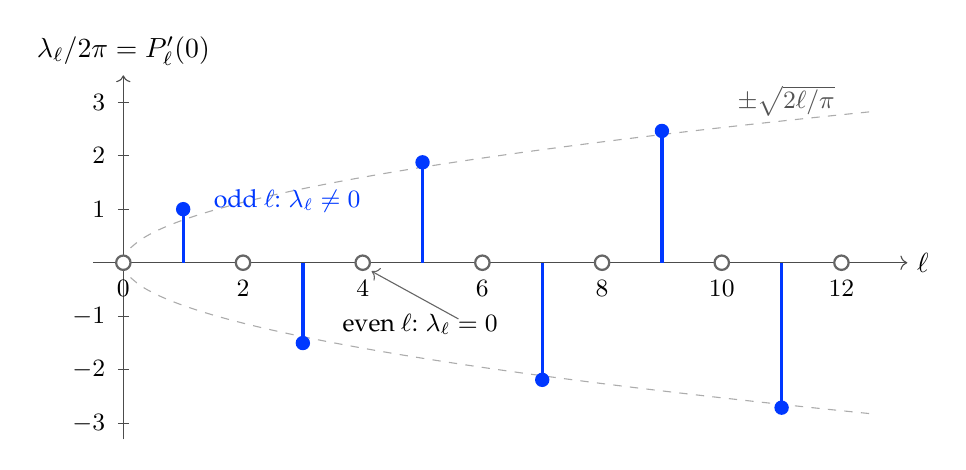
\begin{tikzpicture}[x=0.76cm,y=0.68cm]
  % envelope
  \draw[dashed,gray!65,samples=90,domain=0.12:12.5,smooth,variable=\x]
    plot (\x,{sqrt(2*\x/3.14159)});
  \draw[dashed,gray!65,samples=90,domain=0.12:12.5,smooth,variable=\x]
    plot (\x,{-sqrt(2*\x/3.14159)});
  \node[gray!65!black,font=\small,right] at (10.1,3.02) {$\pm\sqrt{2\ell/\pi}$};

  % axes
  \draw[->,black!70] (-0.5,0) -- (13.1,0) node[right,black] {$\ell$};
  \draw[->,black!70] (0,-3.3) -- (0,3.5)
    node[above,black] {$\lambda_\ell/2\pi=P_\ell'(0)$};
  \foreach \x in {0,2,4,6,8,10,12}{
    \draw[black!70] (\x,-0.09) -- (\x,0.09);
    \node[below,font=\small] at (\x,-0.14) {$\x$};}
  \foreach \y in {-3,-2,-1,1,2,3}{
    \draw[black!70] (-0.09,\y) -- (0.09,\y);
    \node[left,font=\small] at (-0.14,\y) {$\y$};}

  % odd degrees: nonzero, alternating
  \foreach \lev/\val in {1/1, 3/-1.5, 5/1.875, 7/-2.1875, 9/2.4609, 11/-2.707}{
    \draw[very thick,blue] (\lev,0) -- (\lev,\val);
    \fill[blue] (\lev,\val) circle (2.6pt);}

  % even degrees: zero
  \foreach \lev in {0,2,4,6,8,10,12}{
    \draw[fill=white,draw=black!60,thick] (\lev,0) circle (2.6pt);}

  \node[blue,font=\small,right] at (1.35,1.15) {odd $\ell$: $\lambda_\ell\neq0$};
  \draw[->,black!60] (5.6,-1.05) -- (4.15,-0.16);
  \node[font=\small,right] at (3.5,-1.15) {even $\ell$: $\lambda_\ell=0$};
\end{tikzpicture}}
\end{center}

\vspace{-1.6em}
\begin{center}\small
The eigenvalues are zero on even degrees and alternating on odd degrees, with
$|\lambda_\ell|\sim 2\sqrt{2\pi\ell}$.
\end{center}

% \smallskip
\begin{center}
  \begin{tabular}{lcc}
    \toprule
    & \textbf{even modes} & \textbf{odd modes}\\
    \midrule
    Funk transform $\cF$ & \cellcolor{keep}isomorphism & \cellcolor{drop}kernel\\
    $G$-transform $\cG$  & \cellcolor{drop}kernel      & \cellcolor{keep}isomorphism\\
    \bottomrule
  \end{tabular}
\end{center}

\begin{center}\small
Complementary: $\Cinf(\Sph^2)=\ker\cF\oplus\ker\cG$.
\end{center}
}

% =============================================================================
% 7. REGULARITY  (column 3, bottom)
% =============================================================================
\headerbox{\textcolor{white}{7.} Regularity and inversion}{name=reg,column=3,below=harm,above=bottom}{\small
For odd $\ell$,
\vspace{-0.9em}
\[ |\lambda_\ell|\asymp\ell^{1/2}\asymp\big(1+\ell(\ell+1)\big)^{1/4}. \]
% so on the odd subspace $G$ behaves like $(-\Delta_{\Sph^2})^{1/4}$: 
Thus, on the odd subspace, $\cG$ has Sobolov scaling of an operator of order $1/2$.

\medskip
Consequently, for every $s\in\mathbb R$,
\vspace{-0.6em}
\[ \cG:H^{s+1/2}_{\odd}(\Sph^2)\longrightarrow H^{s}_{\odd}(\Sph^2) \]
is an isomorphism, with two-sided bounds
\vspace{-0.3em}
\[ \norm{\cG f}_{H^{s}}\asymp\norm{f}_{H^{s+1/2}}. \]

% \smallskip
\begin{center}
  \fcolorbox{blue}{softblue}{\begin{minipage}{0.9\linewidth}\centering
    \textbf{Inversion.} Given $M\in H^{s}_{\odd}(\Sph^2)$, the equation
    \[ \cG N=M \]
    has a \emph{unique} odd solution $N\in H^{s+1/2}_{\odd}(\Sph^2)$, and
    \[ \norm{N}_{H^{s+1/2}}\lesssim\norm{M}_{H^{s}} . \]
  \end{minipage}}
\end{center}

\medskip
Therefore, $\cG N=M$ gains half a derivative over the data and the even part of $N$ is never determined, since it lies in $\ker\cG$.

% \medskip
% \textbf{Takeaway.} By exploiting the symmetry of these integral-geometric operators, we can explicit spectral multipliers $\lambda_\ell$. Allowing us to compute the kernels and  asymptotics to understand the Sobolev regularity.

}

\headerbox{References}{name=references,column=3, above=bottom}{
\renewcommand{\section}[2]{\vskip 0.05em} % Get rid of the default "References" section title
\nocite{*} % Insert publications even if they are not cited in the poster
\footnotesize{ % Reduce the font size in this block
\bibliographystyle{unsrt}
\bibliography{sources} % Use sample.bib as the bibliography file
}
\medskip
}

\end{poster}
\end{document}
